\documentclass[12pt]{article}


\usepackage{amssymb, xcolor, hyperref}
\usepackage{amsmath}
\usepackage{fullpage}
\usepackage{epsfig}
\usepackage{epstopdf}
\everymath{\displaystyle}
\usepackage{enumerate}

\newif\ifans

\anstrue

\begin{document}

\begin{center}
\underline{\LARGE{Vector Valued Functions}}
\end{center}

\noindent SUGGESTED REFERENCE MATERIAL:

\bigskip

\noindent As you work through the problems listed below, you should reference Chapters 12.1 \& 12.2 of the recommended textbook (or the equivalent chapter in your alternative textbook/online resource) and your lecture notes.

\bigskip

\noindent EXPECTED SKILLS:

\begin{itemize}

\item Be able to find the domain of vector-valued functions. 

\item Be able to describe, sketch, and recognize graphs of vector-valued functions (parameterized curves).

\item Know how to differentiate vector-valued functions. And, consequently, be able to find the tangent line to a curve (as a vector equation or as a set of parametric equations). 

\item Be able to determine angles between tangent lines.

\item Know how to use differentiation formulas involving cross-products and dot products. 

\item Be able to evaluate indefinite and definite integrals of vector-valued functions as well as solve vector initial-value problems.

\end{itemize}

\noindent PRACTICE PROBLEMS:

\medskip

\begin{enumerate}

\item For each of the following, determine the domain of the given function.

\begin{enumerate}

\item ${\bf r}(t)=t^2\text{ }{\bf i}+\sqrt{1-t}\text{ }{\bf j}-\frac{1}{t}\text{ }{\bf k}$

\ifans{\fbox{$(-\infty,0)\cup(0,1]$}} \fi

\item ${\bf r}(t)=\left\langle \ln{(t+1)}, \frac{1}{e^t-2}, t\right\rangle$

\ifans{\fbox{$(-1,\ln2)\cup(\ln2,\infty)$}} \fi

\item ${\bf r}(t)=\cos{(t)}{\bf i}+\sin{(t)}{\bf j}+5{\bf k}$

\ifans{\fbox{$(-\infty,\infty)$}} \fi

\end{enumerate}

\newpage

\item Consider the curve $C: {\bf r}(t)=\langle -5+t,-4+2t\rangle$, shown below.

\begin{center}
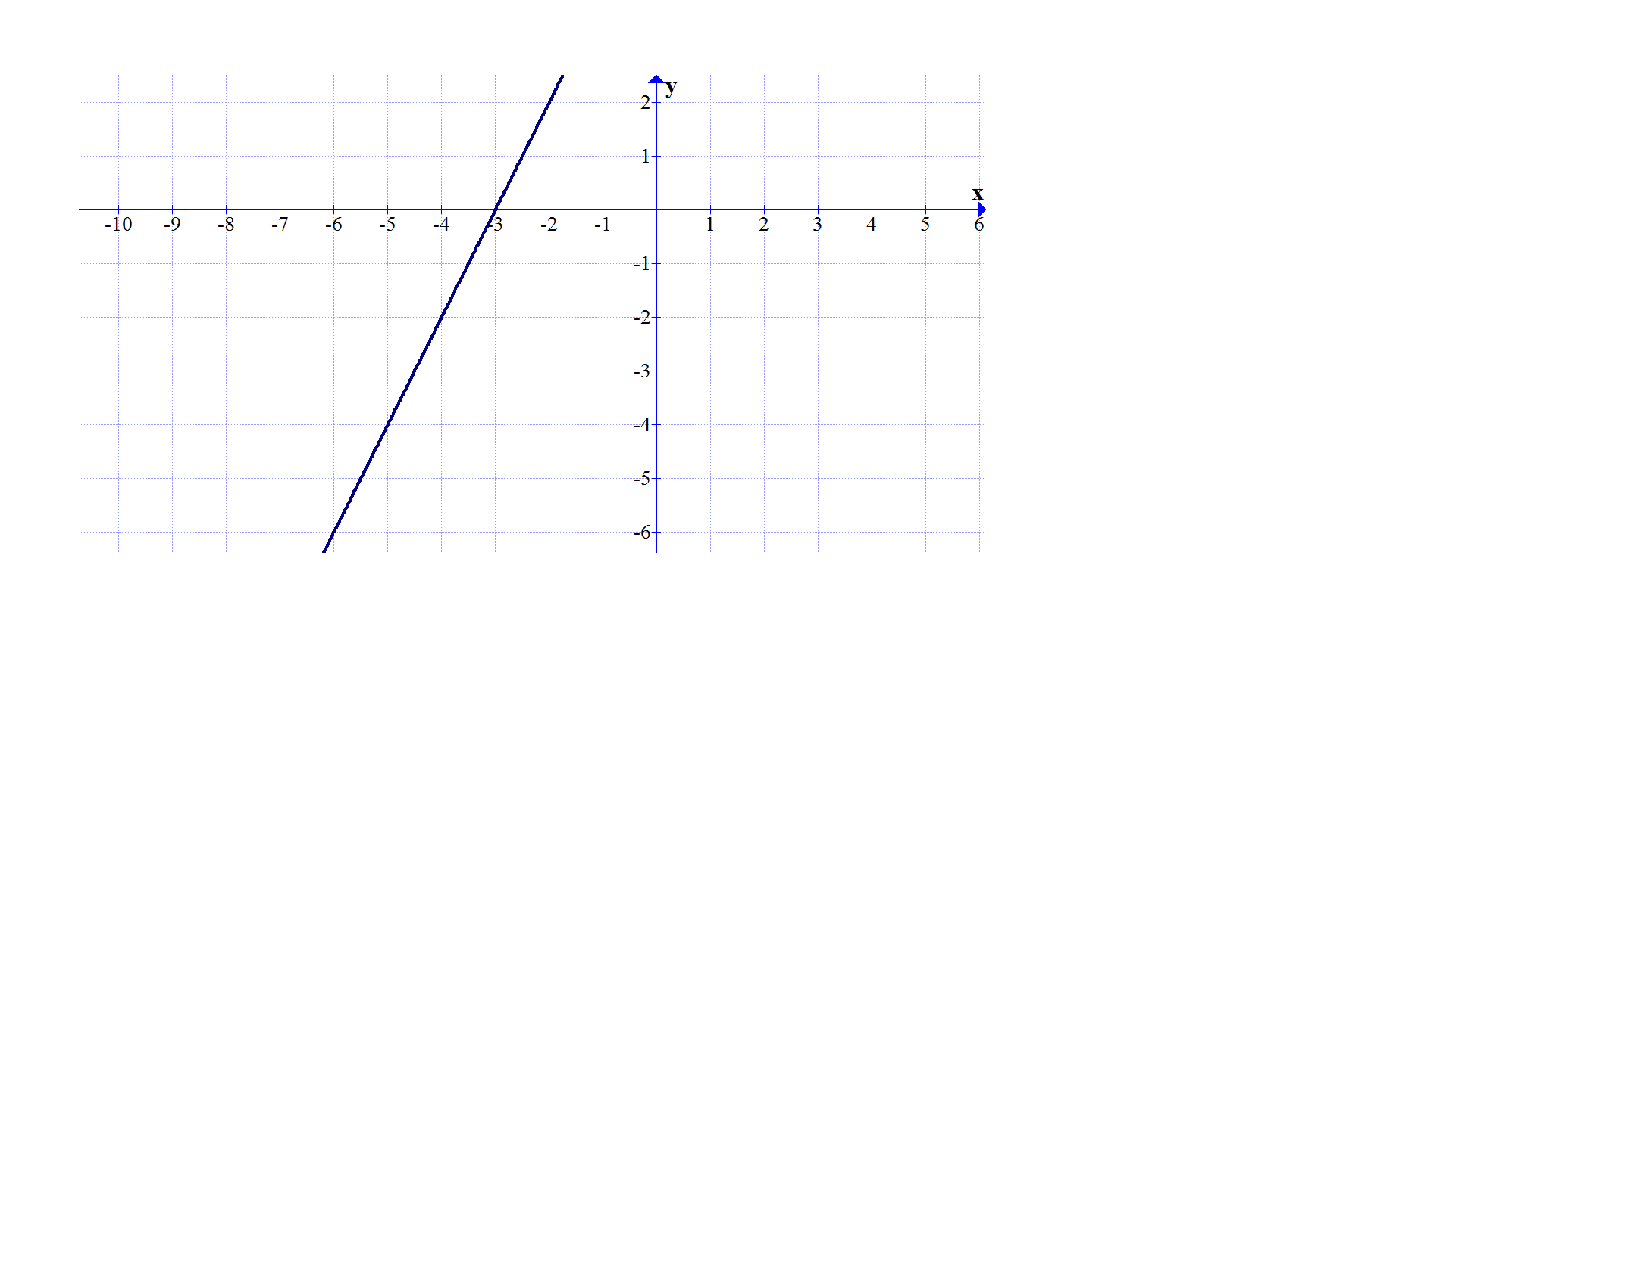
\includegraphics[scale=0.58]{line.pdf}
\end{center}

\begin{enumerate}

\item Sketch the following position vectors: ${\bf r}(-1)$, ${\bf r}(0)$, ${\bf r}(1)$, ${\bf r}(2)$,  and ${\bf r}(3)$. 

\ifans{\fbox{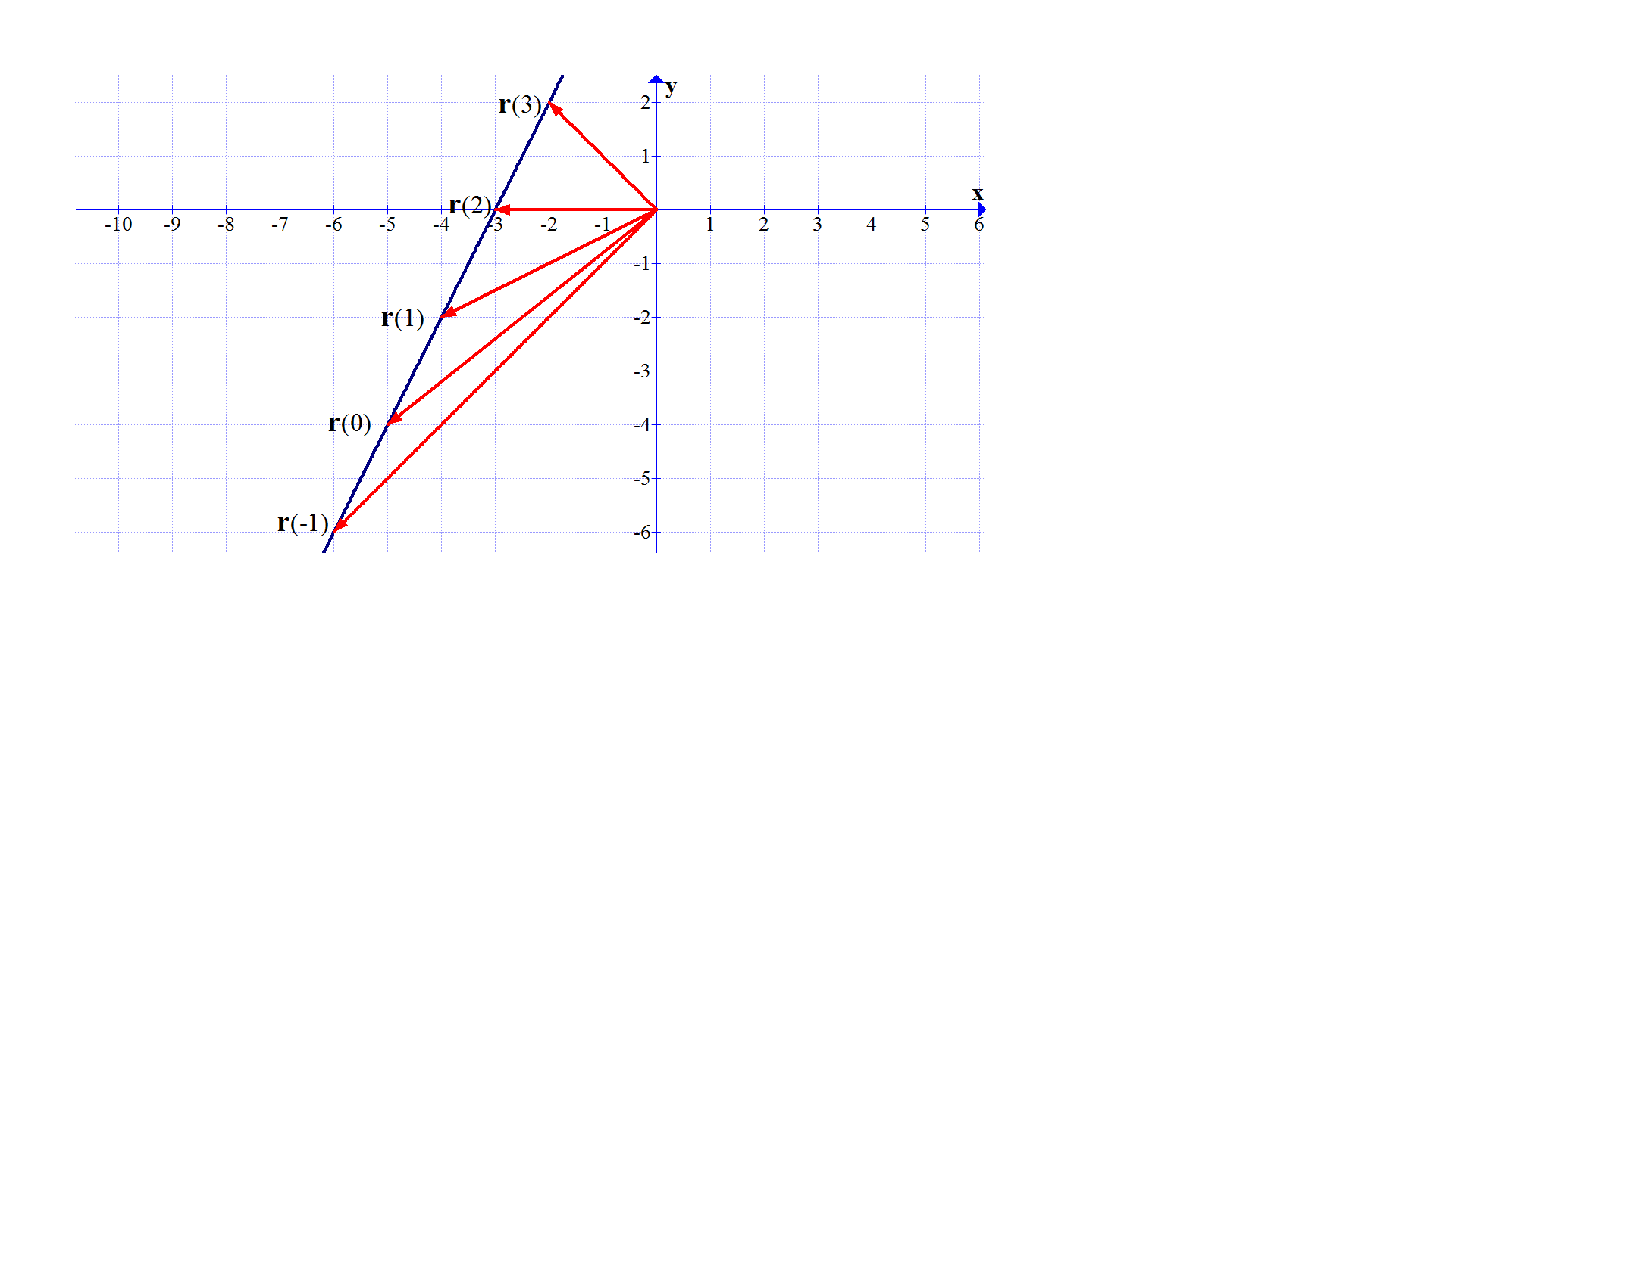
\includegraphics[scale=0.4]{line_a.pdf}}} \fi

\item Indicate the orientation of the curve (i.e., the direction or increasing $t$).

\ifans{\fbox{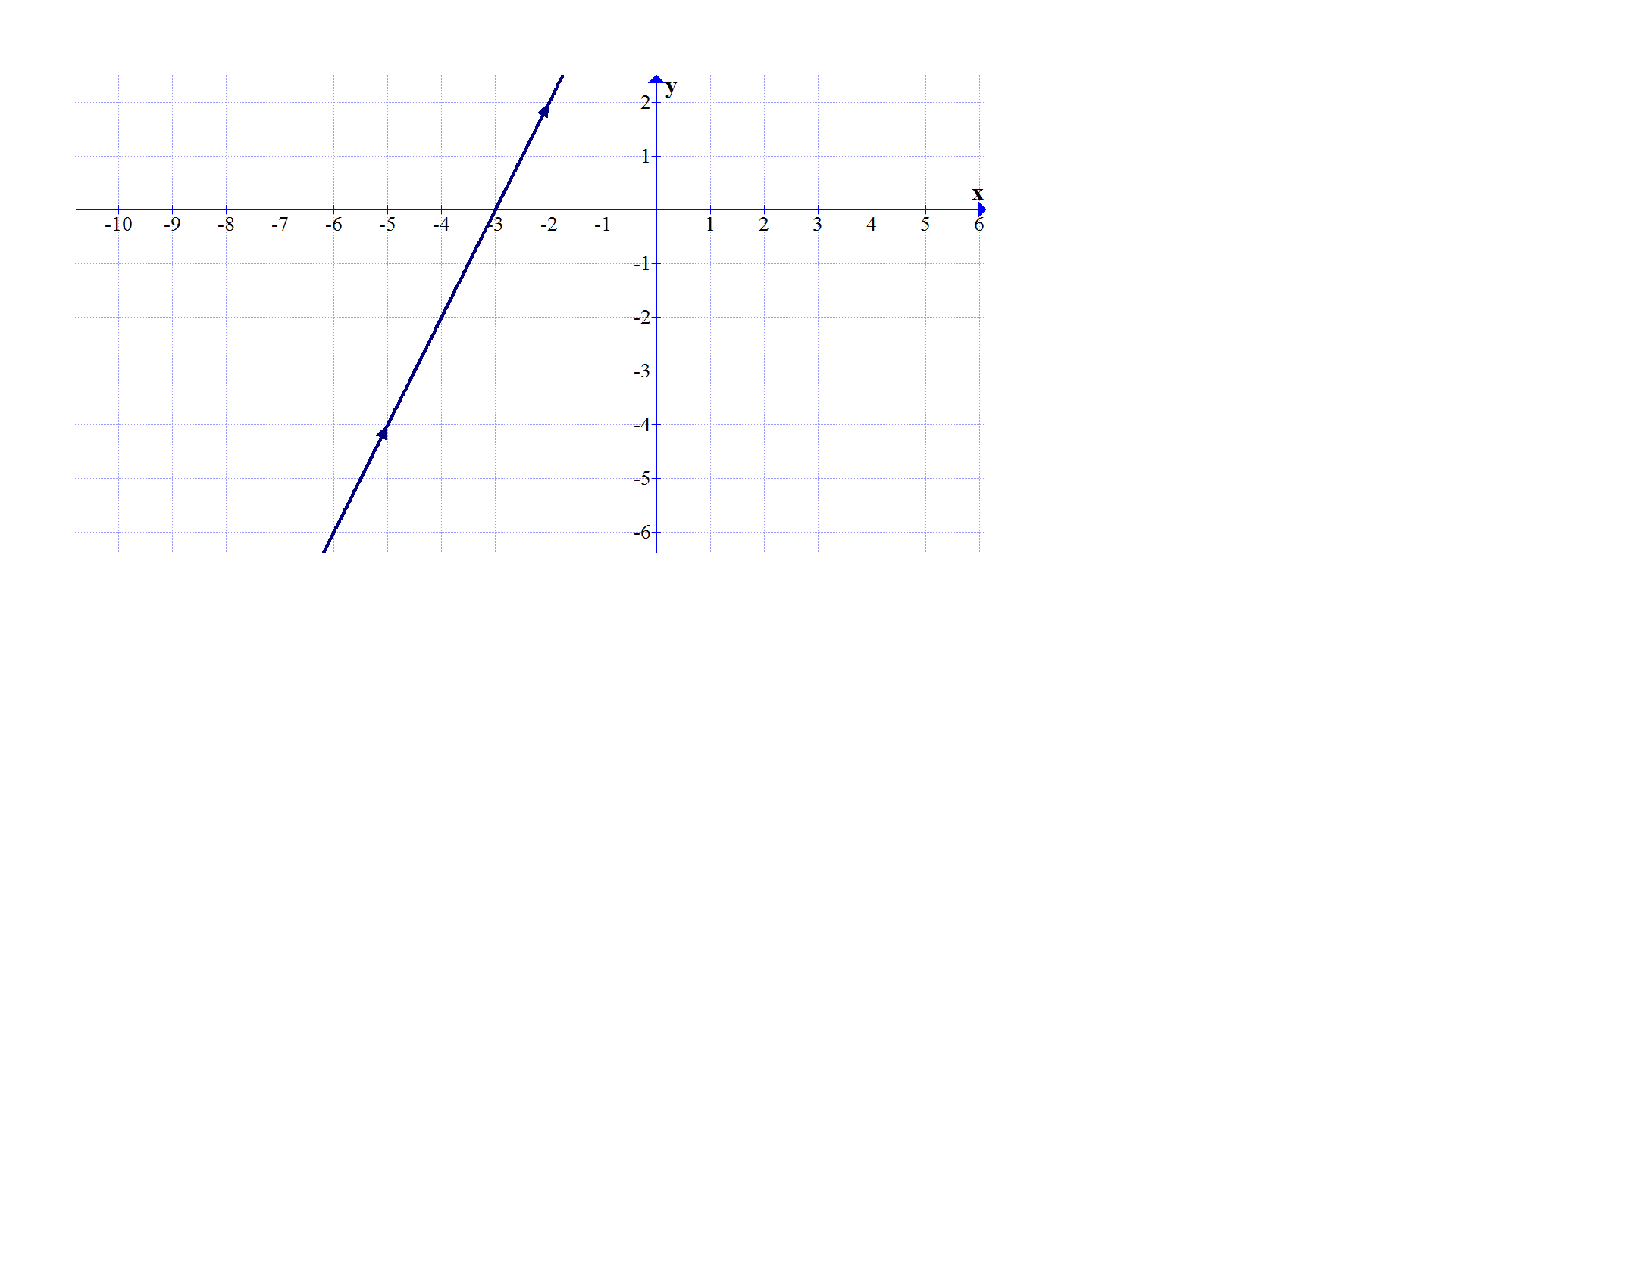
\includegraphics[scale=0.4]{line_b.pdf}}} \fi

\end{enumerate}

\item Sketch the following vector valued functions.  Also, describe the curve in words.

\begin{enumerate}

\item $\overrightarrow{r}(t)=\langle 4\cos{t}, 4\sin{t}, 5 \rangle$, $0 \leq t \leq 4\pi$

\ifans{\fbox{\parbox{1\linewidth}{The curve is a circle in the $z=5$ plane which has a radius of 4 and a center at $(0,0,5)$, traversed twice counterclockwise.
\begin{center}
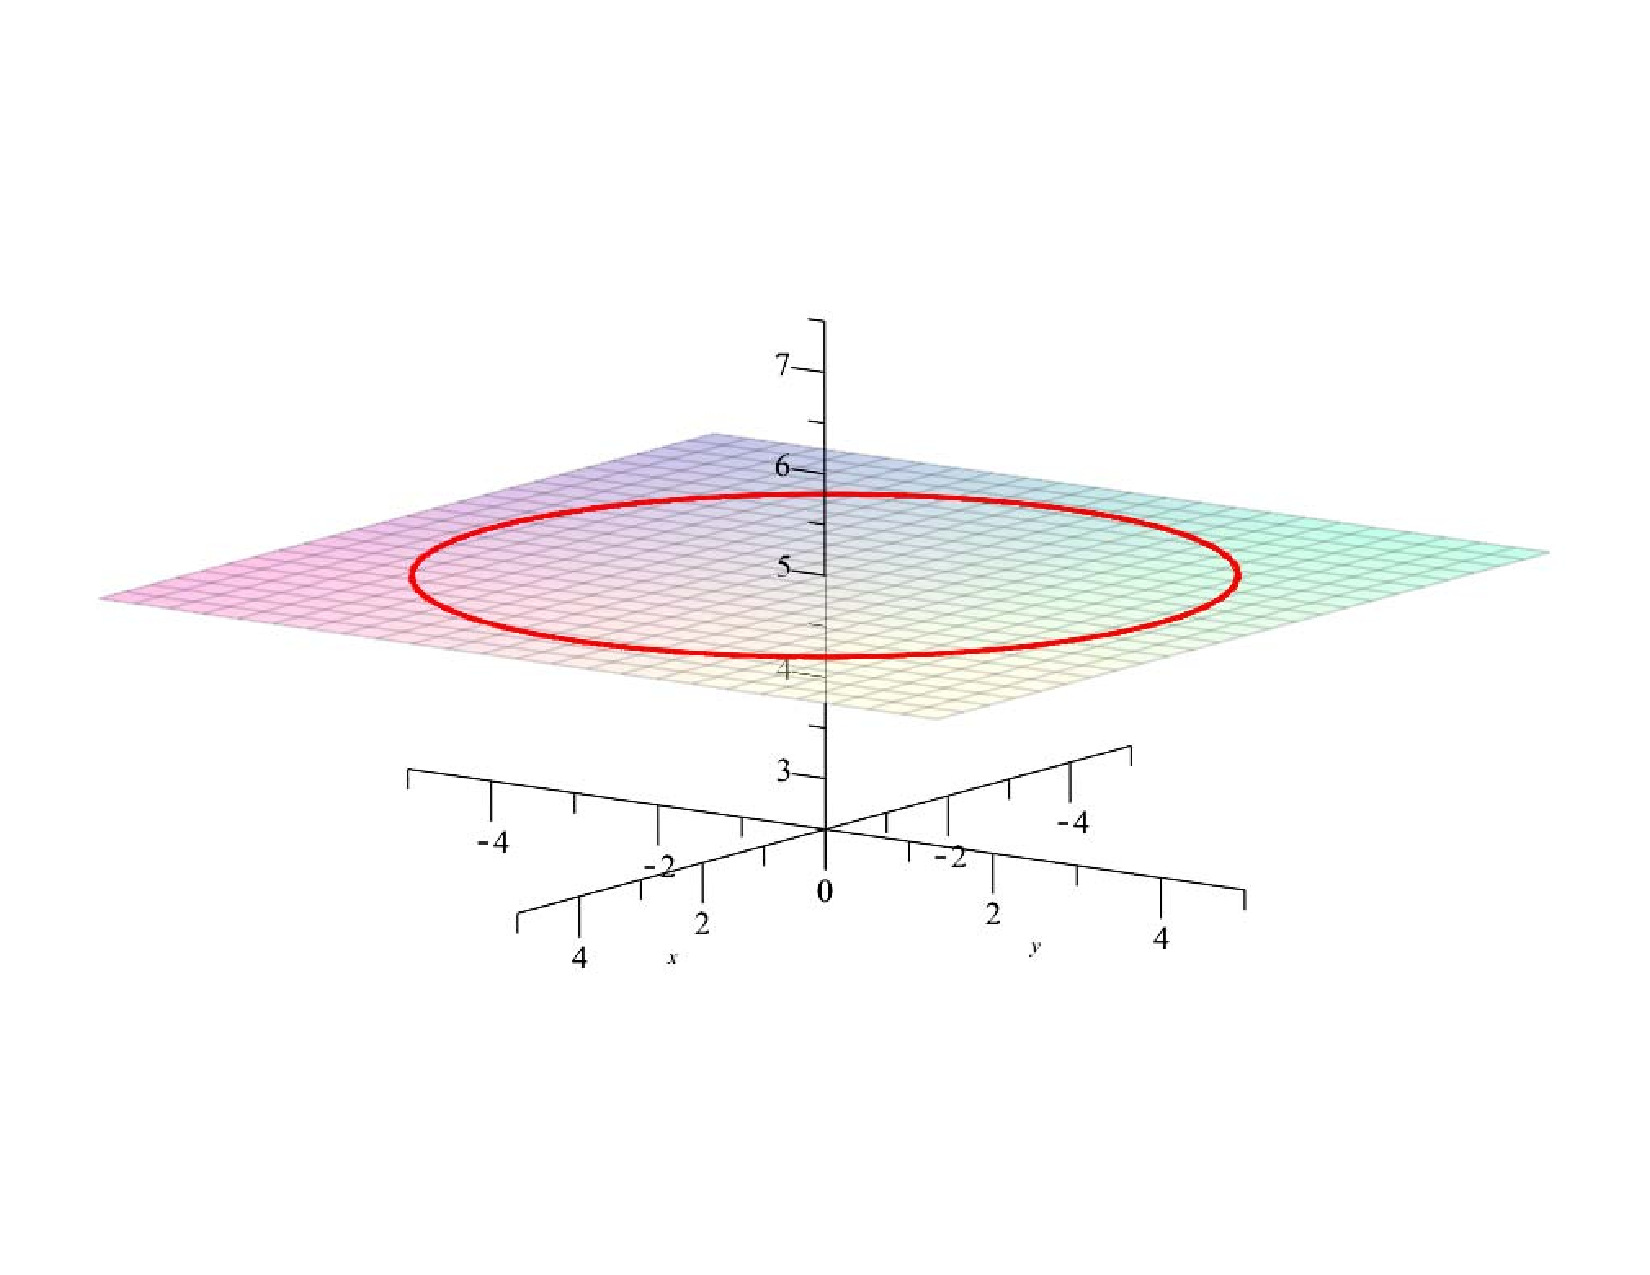
\includegraphics[scale=0.25]{curve1.pdf}
\end{center}}}} \fi

\item $\overrightarrow{r}(t)=\langle 4\cos{t}, 4\sin{t}, t \rangle$, $0 \leq t \leq 4\pi$.

\ifans{\fbox{\parbox{1\linewidth}{The curve is a helix on the cylinder $x^2+y^2=16$ which climbs from the point $(4,0,0)$ to the point $(4,0,4\pi)$
\begin{center}
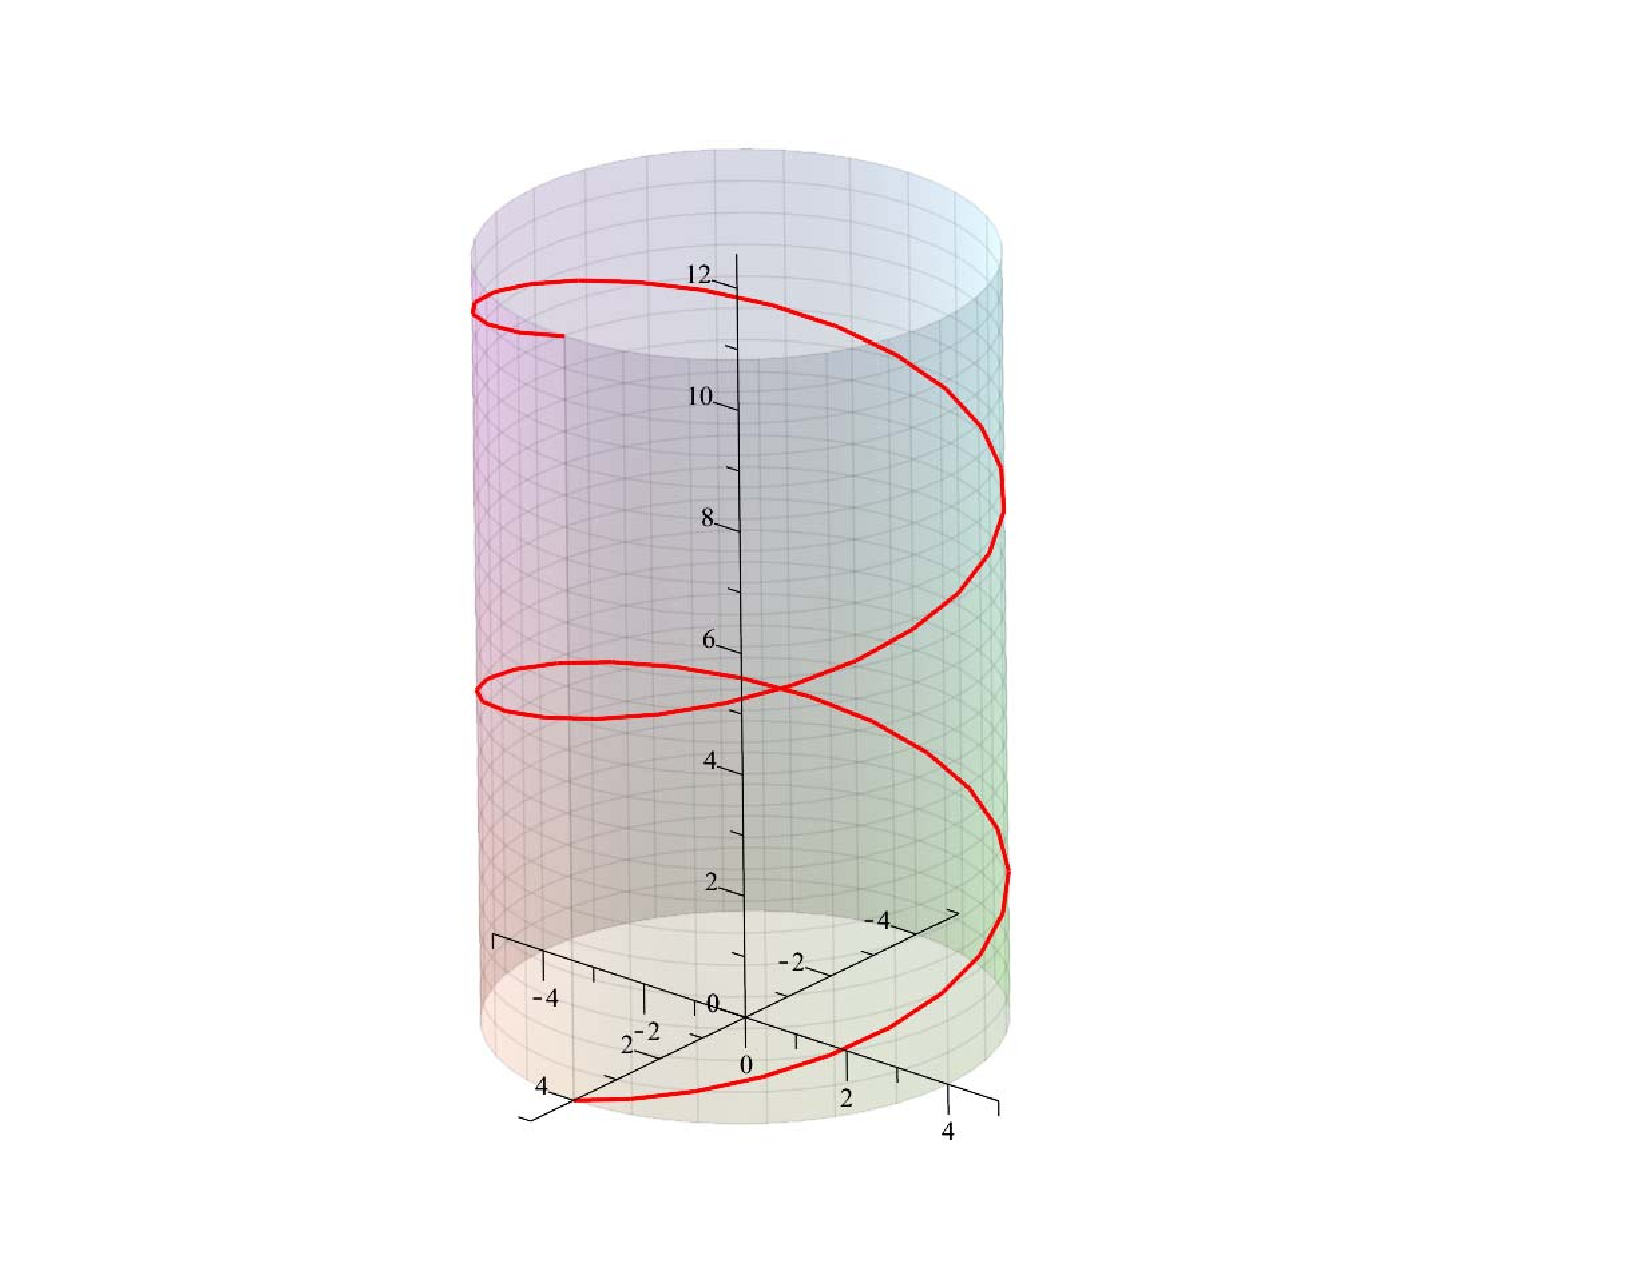
\includegraphics[scale=0.25]{curve2.pdf}
\end{center}}}} \fi

\end{enumerate}

\item Consider ${\bf r}(t)=\langle t,t^2\rangle$

\begin{enumerate}

\item Sketch ${\bf r}(t)$ and indicate the direction of increasing $t$.

\item On your sketch, draw ${\bf r}(1)$ and ${\bf r}^{\prime}(1)$.

\ifans{\fbox{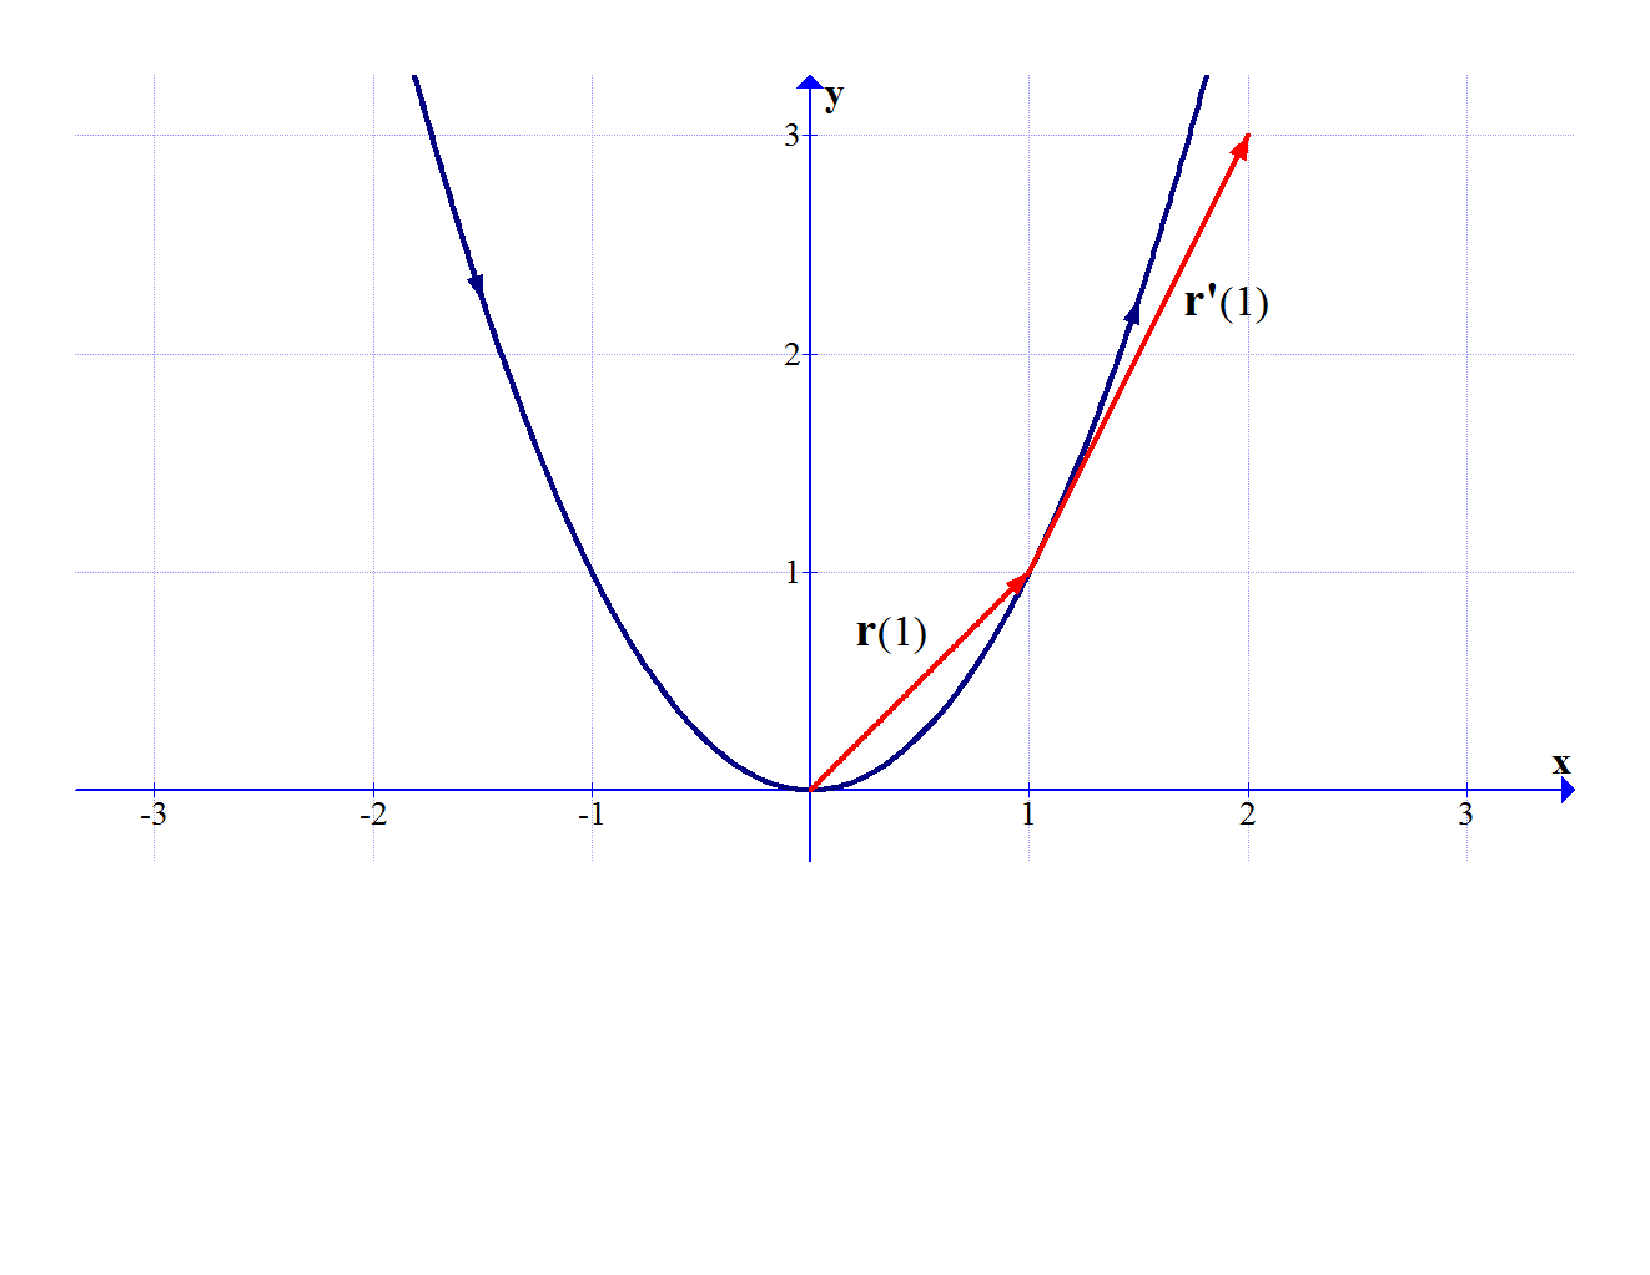
\includegraphics[scale=0.3]{parabola.pdf}}} \fi

\end{enumerate}

\item Consider ${\bf r}(t)=\langle 3\cos{t},2\sin{t}\rangle$

\begin{enumerate}

\item Sketch ${\bf r}(t)$ and indicate the direction of increasing $t$.

\item On your sketch, draw ${\bf r}(\pi)$ and ${\bf r}^{\prime}(\pi)$.

\ifans{\fbox{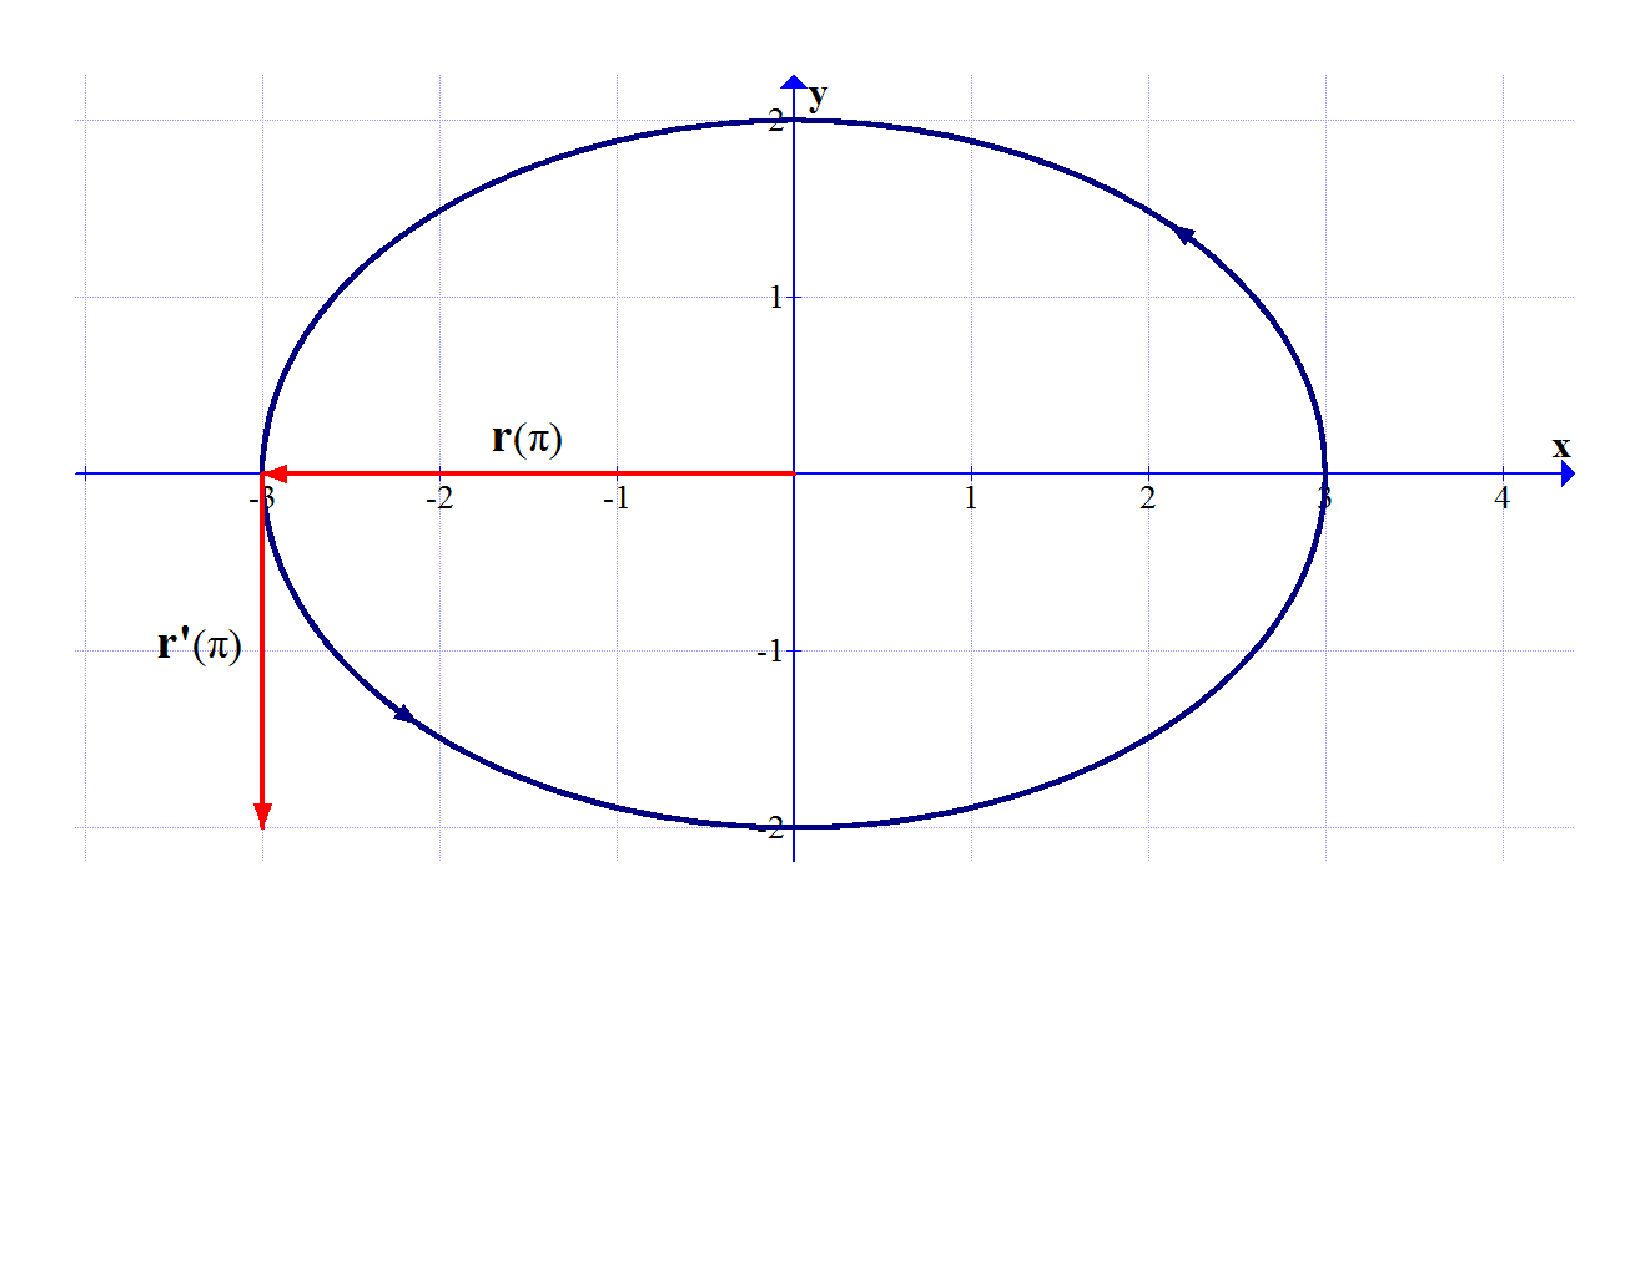
\includegraphics[scale=0.3]{ellipse.pdf}}} \fi

\end{enumerate}

\item For each of the following, find an equation of the line which is tangent to the given curve at the indicated point.

\begin{enumerate}

\item ${\bf r}(t)=\left\langle \ln{t}, 2\sqrt{t}, t^2\right\rangle$ at $(x,y,z)=(0,2,1)$

\ifans{\fbox{$\overrightarrow{\ell}(t)=\langle 0,2,1 \rangle + t\langle 1, 1, 2\rangle$}} \fi

\item ${\bf r}(t)=\left\langle \sin{t},\cos{t},\tan{t}\right\rangle$ when $t=\pi$

\ifans{\fbox{$\overrightarrow{\ell}(t)=\langle 0,-1,0 \rangle + t\langle -1, 0, 1\rangle$}} \fi

\end{enumerate}

\item Find all points on the curve ${\bf r}(t)=t{\bf i}+t^2{\bf j}+t^3{\bf k}$ where its tangent line is parallel to the vector $2{\bf i}+8{\bf j}+24{\bf k}$.

\ifans{\fbox{\parbox{1\linewidth}{The tangent line will be parallel to the given vector when $t=2$ which corresponds to the point $(x,y,z)=(2,4,8)$; Detailed Solution: \textcolor{blue}{\href{http://www.math.drexel.edu/classes/Calculus/resources/Math200HW/Solutions/08_200_Vector_Functions_07.pdf}{Here}} }}} \fi

\item The following vector valued functions describe the paths of two bugs flying in space.  

$${\bf r_1}(t)=\langle t^2, 2t+3, t^2\rangle$$
$${\bf r_2}(t)=\langle 5t-6, t^2, 9\rangle$$

At some moment in time, the two bugs collide.

\begin{enumerate}

\item Determine the moment in time when the bugs collide as well as the location in space where the bugs collide.

\ifans{\fbox{\parbox{1\linewidth}{The bugs intersect when $t=3$.  This corresponds to the point $(x,y,z)=(9,9,9)$. Detailed Solution: \textcolor{blue}{\href{http://www.math.drexel.edu/classes/Calculus/resources/Math200HW/Solutions/08_200_Vector_Functions_08.pdf}{Here}}}}} \fi

\item What is the angle between their paths at the point of collision?

\ifans{\fbox{$\cos^{-1}\left(\frac{42}{\sqrt{76}\sqrt{61}}\right)$; Detailed Solution: \textcolor{blue}{\href{http://www.math.drexel.edu/classes/Calculus/resources/Math200HW/Solutions/08_200_Vector_Functions_08.pdf}{Here}}}} \fi

\end{enumerate}

\item Prove the following theorem:

{\bf Theorem:} \emph{If $\overrightarrow{r}(t)$ is a differentiable vector valued function in 2-space or 3-space, and if $\|\overrightarrow{r}(t)\|$ is constant for all $t$, then $\overrightarrow{r}(t)\cdot\overrightarrow{r}^{\prime}(t)=0$.  That is, $\overrightarrow{r}(t)$ and $\overrightarrow{r}^{\prime}(t)$ are orthogonal vectors for all $t$.}

(Hint: $\|\overrightarrow{r}(t)\|^2=\overrightarrow{r}(t)\cdot\overrightarrow{r}(t)$)

\ifans{\fbox{\parbox{1\linewidth}{Suppose $\|\overrightarrow{r}(t)\|=k$, where $k$ is constant.  Then:
\begin{align*}
\|\overrightarrow{r}(t)\|^2&=k^2\\
\overrightarrow{r}(t)\cdot\overrightarrow{r}(t)&=k^2\\
\frac{d}{dt}\left[\overrightarrow{r}(t)\cdot\overrightarrow{r}(t)\right]&=\frac{d}{dt}\left(k^2\right)\\
\overrightarrow{r}(t)\cdot \overrightarrow{r}^{\prime}(t)+\overrightarrow{r}^{\prime}(t)\cdot \overrightarrow{r}(t)&=0\\
2\left[\overrightarrow{r}(t)\cdot \overrightarrow{r}^{\prime}(t)\right]&=0\\
\overrightarrow{r}(t)\cdot \overrightarrow{r}^{\prime}(t)&=0
\end{align*}
And, the result is proven.
}}} \fi

\item Explain why the following calculation is incorrect:
$$\frac{d}{dt}\left[{\bf r_1}(t)\times{\bf r_2}(t)\right]={\bf r_1}(t)\times {\bf r_2}^{\prime}(t)+{\bf r_2}(t)\times{\bf r_1}^{\prime}(t)$$

\ifans{\fbox{\parbox{1\linewidth}{The order of the terms matters when dealing with cross products.  The correct derivative statement is:
$$\frac{d}{dt}\left[{\bf r_1}(t)\times{\bf r_2}(t)\right]={\bf r_1}(t)\times {\bf r_2}^{\prime}(t)+{\bf r_1}^{\prime}(t)\times{\bf r_2}(t)$$}}} \fi

\item Evaluate the following integrals.

\begin{enumerate}

\item $\int \left[(2t+1)^5{\bf i}-\frac{1}{t}{\bf j}\right]\,dt$

\ifans{\fbox{$\left(\frac{1}{12}(2t+1)^6+c_1\right){\bf i}-(\ln{|t|}+c_2){\bf j}$; i.e., $\left\langle\frac{1}{12}(2t+1)^6,-\ln{|t|}\right\rangle+\overrightarrow{c}$}} \fi

\item $\int \langle \sin{t},\cos{t},\tan{t} \rangle \,dt$

\ifans{\fbox{\parbox{1\linewidth}{$(-\cos{t}+c_1){\bf i}+(\sin{t}+c_2){\bf j}+(\ln{|\sec{t}|}+c_3){\bf k}$; or, equivalently,
$\left\langle -\cos{t}, \sin{t}, \ln{|\sec{t}|}\right\rangle+\overrightarrow{c}$}}} \fi

\item $\int_0^{\ln3} \left[e^t{\bf i}+e^{2t}{\bf j}\right] \,dt$

\ifans{\fbox{$\langle 2,4 \rangle$}} \fi

\end{enumerate}

\item  Evaluate $\int_0^{2\pi} \|{\bf r}^{\prime}(t)\| \,dt$ if ${\bf r}(t)=\langle 3\cos{t}, 3\sin{t} \rangle$.  Interpret your answer geometrically.

\ifans{\fbox{\parbox{1\linewidth}{$6\pi$.  The given curve represents a circle centered at the origin with a radius of 3; this integral gives the arc length (circumference) of the circle.}}} \fi

\item Solve the following vector initial value problems: $\left\{\begin{array}{l}
\frac{d{\bf r}}{dt}=e^{-t}{\bf i}+3t^2{\bf j}\\
\\
{\bf r}(0)=2{\bf i}-8{\bf j}\end{array}\right.$

\ifans{\fbox{${\bf r}(t)=\langle -e^{-t}+3, t^3-8 \rangle$}} \fi

\item A particle moves through 3-space in such a way that its velocity is ${\bf v}(t)=t{\bf i}+t^2{\bf j}+t^3{\bf k}$.  If the particle's initial position at time $t=0$ is $(1,2,3)$, what is the particle's position when $t=1$? (Hint: set up an initial value problem.)

\ifans{\fbox{\parbox{1\linewidth}{The position of the particle at time $t=1$ is $(x,y,z)=\left( \frac{3}{2}, \frac{7}{3}, \frac{13}{4}\right)$.  Detailed Solution: \textcolor{blue}{\href{http://www.math.drexel.edu/classes/Calculus/resources/Math200HW/Solutions/08_200_Vector_Functions_14.pdf}{Here}}}}} \fi

\item Suppose that $C: {\bf r}(t)$ is a smooth vector valued function in 2-space or 3-space defined for $a \leq t \leq b$.  We define the {\bf arc length function} by $$s(t)=\int_{t_0}^t \|{\bf r}^{\prime}(u)\| \,du$$

This function gives the arc length for the part of $C$ between ${\bf r}(t_0)$ and ${\bf r}(t)$.

\begin{enumerate}

\item Compute the arc length function for the helix ${\bf r}(t)=\cos{t} {\bf i}+\sin{t} {\bf j}+t {\bf k}$ which gives the length of the curve from $t_0=0$ to an arbitrary $t$.

\ifans{\fbox{$s=\sqrt{2}t$}} \fi

\item Use your answer from part (a) to reparameterize the helix with respect to arc length. (In other words, express the curve $C$ as ${\bf r}(s)$.)

\ifans{\fbox{${\bf r}(s)=\cos\left(\frac{s}{\sqrt{2}}\right){\bf i}+\sin\left(\frac{s}{\sqrt{2}}\right){\bf j}+\frac{s}{\sqrt{2}}{\bf k}$}} \fi

\item Compute ${\bf r}^{\prime}(s)$ and $\|{\bf r}^{\prime}(s)\|$

\ifans{\fbox{\parbox{1\linewidth}{${\bf r}^{\prime}(s)=-\frac{1}{\sqrt{2}}\sin\left(\frac{s}{\sqrt{2}}\right){\bf i}+\frac{1}{\sqrt{2}}\cos\left(\frac{s}{\sqrt{2}}\right){\bf j}+\frac{1}{\sqrt{2}}{\bf k}$ and $\|{\bf r}^{\prime}(s)\|=1$\\
In fact, whenever a curve is parameterized in terms of arc length, it can be shown using the chain rule that all tangent vectors will be unit tangent vectors.
}}} \fi

\end{enumerate}

\newpage

\item From the ground, a projectile is shot upward at an angle of $\alpha$ with the horizontal, $\left(0<\alpha<\frac{\pi}{2}\right)$, at an initial speed of $v_0$ meters/second, as demonstrated in the diagram below.

\begin{center}
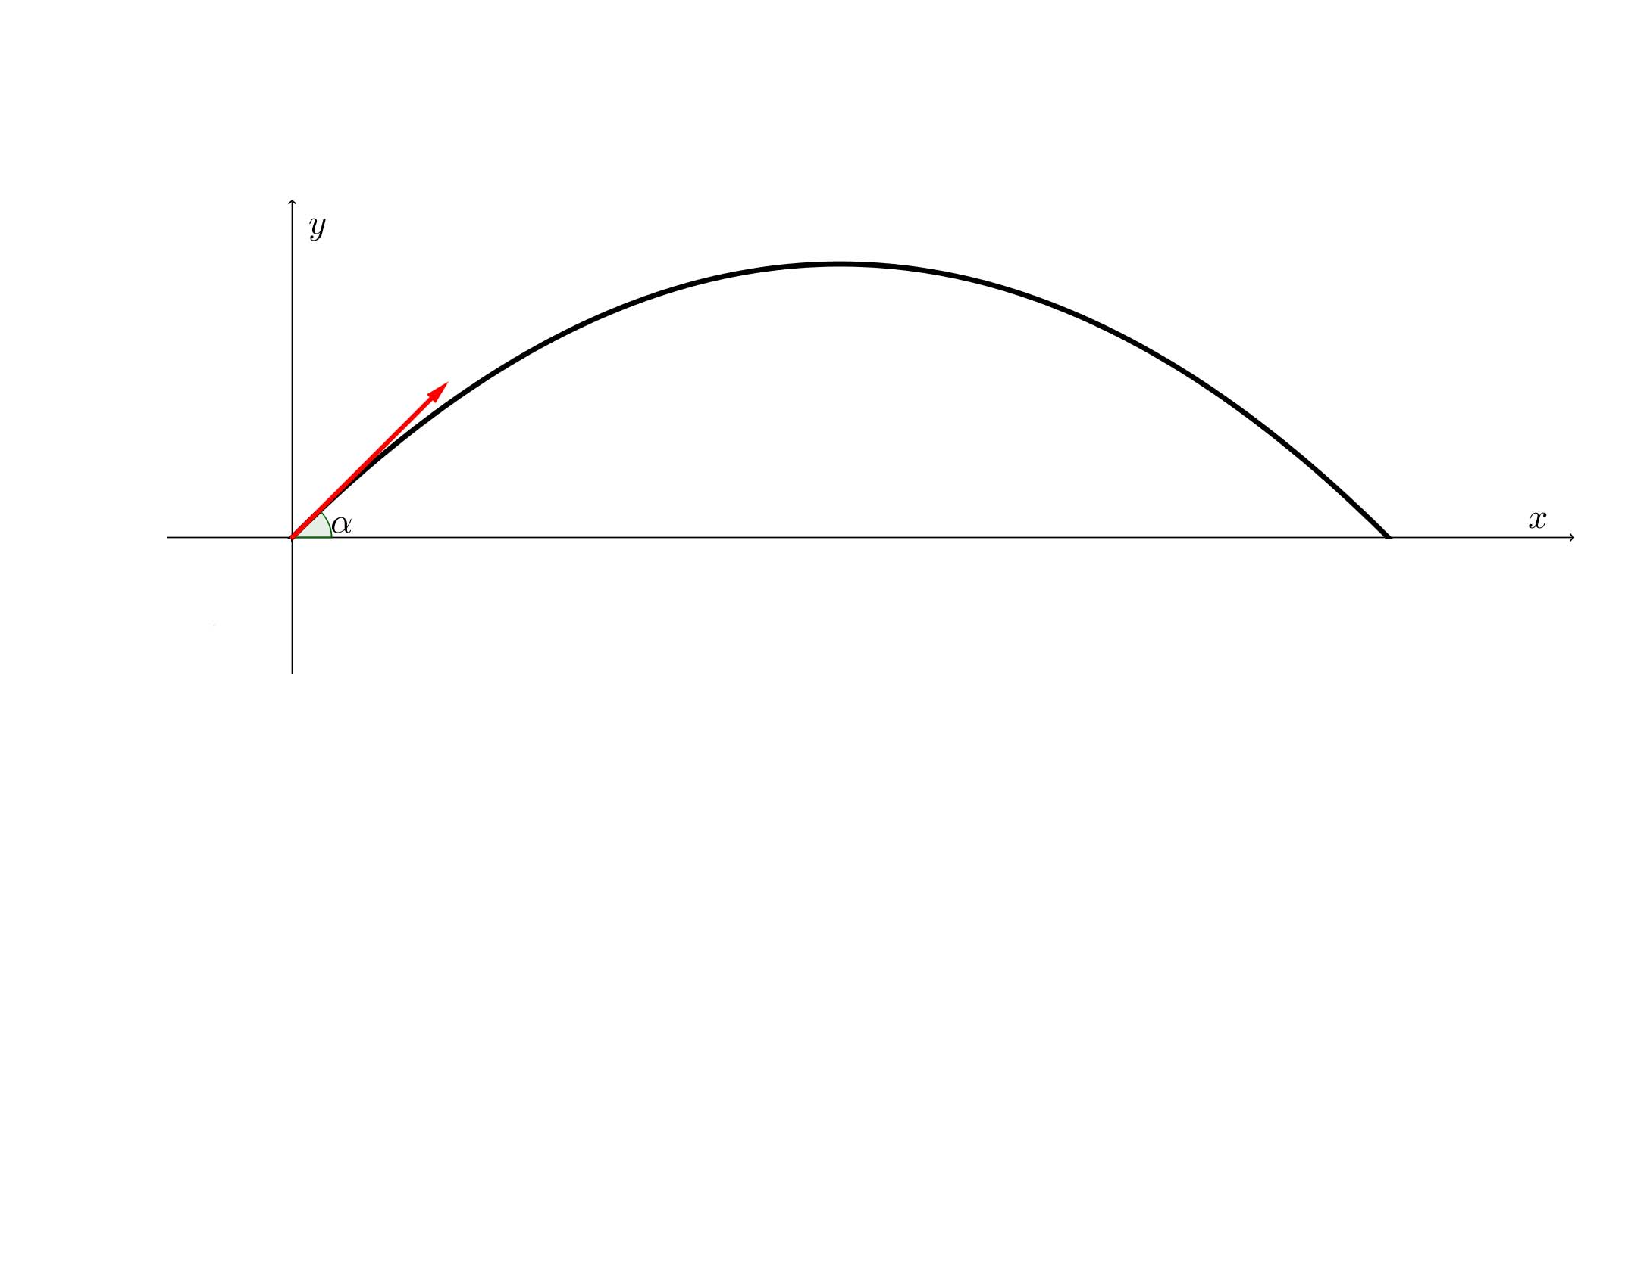
\includegraphics[scale=0.5]{projectile.pdf}
\end{center}

You should make the following assumptions:

\begin{itemize}

\item The mass of the object, $m$, is constant.

\item The only force acting on the object after it is launched is the force of gravity, $g$.  Ignore air resistance and assume that the force of gravity is constant.

\end{itemize}

\begin{enumerate}

\item Set up an initial value problem which can be used to find ${\bf r}(t)$, a vector valued function that gives the position of the particle at time $t$.

\ifans{\fbox{$\left\{\begin{array}{l}
{\bf a}(t)=\frac{d^2{\bf r}}{dt^2}=\langle 0, -g \rangle\\
\\
{\bf v}(0)={\bf r}^{\prime}(0)=\langle v_0\cos{\alpha}, v_0\sin{\alpha} \rangle\\
\\
{\bf r}(0)= \langle 0,0 \rangle\end{array}\right.$}} \fi

\item Solve your initial value problem from part (a) to determine ${\bf r}(t)$.

\ifans{\fbox{${\bf r}(t)=\left\langle v_0(\cos{\alpha})t, -\frac{1}{2}gt^2+v_0(\sin\alpha)t\right\rangle$}} \fi

\item Verify that the trajectory of the projectile is a parabola.

\ifans{\fbox{\parbox{1\linewidth}{We can express the trajectory of the projectile (from part b) parametrically:\\
$$\left\{\begin{array}{l}
x=v_0(\cos{\alpha})t\\
\\
y=-\frac{1}{2}gt^2+v_0(\sin\alpha)t\end{array}\right.$$

Notice that if we solve the first equation for $t$, we get $t=\frac{x}{v_0\cos{\alpha}}$.  (It was OK to do this division since we had some non-zero instantaneous speed $v_0$ and $\cos{\alpha}\neq 0$ for $0 < \alpha <\frac{\pi}{2}$).  Then, plugging this into the second equation, we get:
\begin{align*}
y&=-\frac{1}{2}g\left(\frac{x}{v_0\cos{\alpha}} \right)^2+v_0(\sin\alpha)\left(\frac{x}{v_0\cos{\alpha}}\right)\\
&=-\frac{g}{2(v_0\cos\alpha)^2}x^2+(\tan{\alpha})x\\
&=-Ax^2+Bx
\end{align*}
where $A$ is the constant $\frac{g}{2(v_0\cos\alpha)^2}$ and $B$ is the constant $\tan\alpha$.  Thus, the trajectory is parabolic.
}}} \fi

\item What is the flight time of the projectile?

\ifans{\fbox{\parbox{1\linewidth}{We can find the value of $t$ for which the projectile returns to the ground by setting $y=0$ in the parametric representation of the trajectory.
\begin{align*}
y&=0\\
-\frac{1}{2}gt^2+v_0(\sin\alpha)t &=0\\
-t\left(\frac{1}{2}gt-v_0\sin\alpha\right)&=0
\end{align*}
which happens when $t=0$ and when $t=\frac{2v_0\sin\alpha}{g}$
}}} \fi

\item What is the range of the projectile?

\ifans{\fbox{\parbox{1\linewidth}{To find the range, we need to determine the $x$ coordinate at the time when the projectile returns to the ground.  Specifically, the range is: $$x\left(\frac{2v_0\sin\alpha}{g}\right)=v_0(\cos\alpha)\left(\frac{2v_0\sin\alpha}{g}\right)=\frac{v_0^2\sin{(2\alpha)}}{g}$$
}}} \fi

\newpage

\item What angle $\alpha$ maximizes the range?

\ifans{\fbox{\parbox{1\linewidth}{In part (e), we have already computed the range to be $\frac{v_0^2}{g}\sin{(2\alpha)}$.  This is maximized when $\sin(2\alpha)=1$; i.e., when $\alpha =\frac{\pi}{4}$
}}} \fi

\end{enumerate}

\item Suppose that $C:{\bf r}(t)$ is a curve in 2-space or 3-space and that $\|{\bf r}^{\prime}(t)\|\neq 0$.  We define the following vectors:
\begin{itemize}

\item The \underline{Unit Tangent Vector} to $C$ at $t$ is ${\bf T}(t)=\frac{{\bf r}^{\prime}(t)}{\|{\bf r}^{\prime}(t)\|}$.

\item The \underline{Principal Unit Normal Vector} to $C$ at $t$ is ${\bf N}(t)=\frac{{\bf T}^{\prime}(t)}{\|{\bf T}^{\prime}(t)\|}$.

\item The \underline{Unit Binormal Vector} to $C$ at $t$ is ${\bf B}(t)={\bf T}(t)\times {\bf N}(t)$.

\end{itemize}

The coordinate system determined at the point $t$ by ${\bf T}(t)$, ${\bf N}(t)$, and ${\bf B}(t)$ is called the \underline{Frenet Frame} or the \underline{{\bf TNB} Frame}.

\begin{enumerate}

\item Explain why ${\bf T}(t)$, ${\bf N}(t)$, and ${\bf B}(t)$ are all mutually othogonal.

\ifans{\fbox{\parbox{1\linewidth}{${\bf N}(t)\perp {\bf T}(t)$ by problem 9.  ${\bf B}(t) \perp {\bf N}(t)$ and ${\bf B}(t) \perp {\bf T}(t)$ because for any vectors in three space ${\bf v} \cdot ({\bf v}\times{\bf w})=0$ and ${\bf w} \cdot ({\bf v}\times{\bf w})=0$}}} \fi

\item Consider the helix described by ${\bf r}(t)=\langle 2 \cos{t}, t, 2\sin{t} \rangle$.

\begin{center}
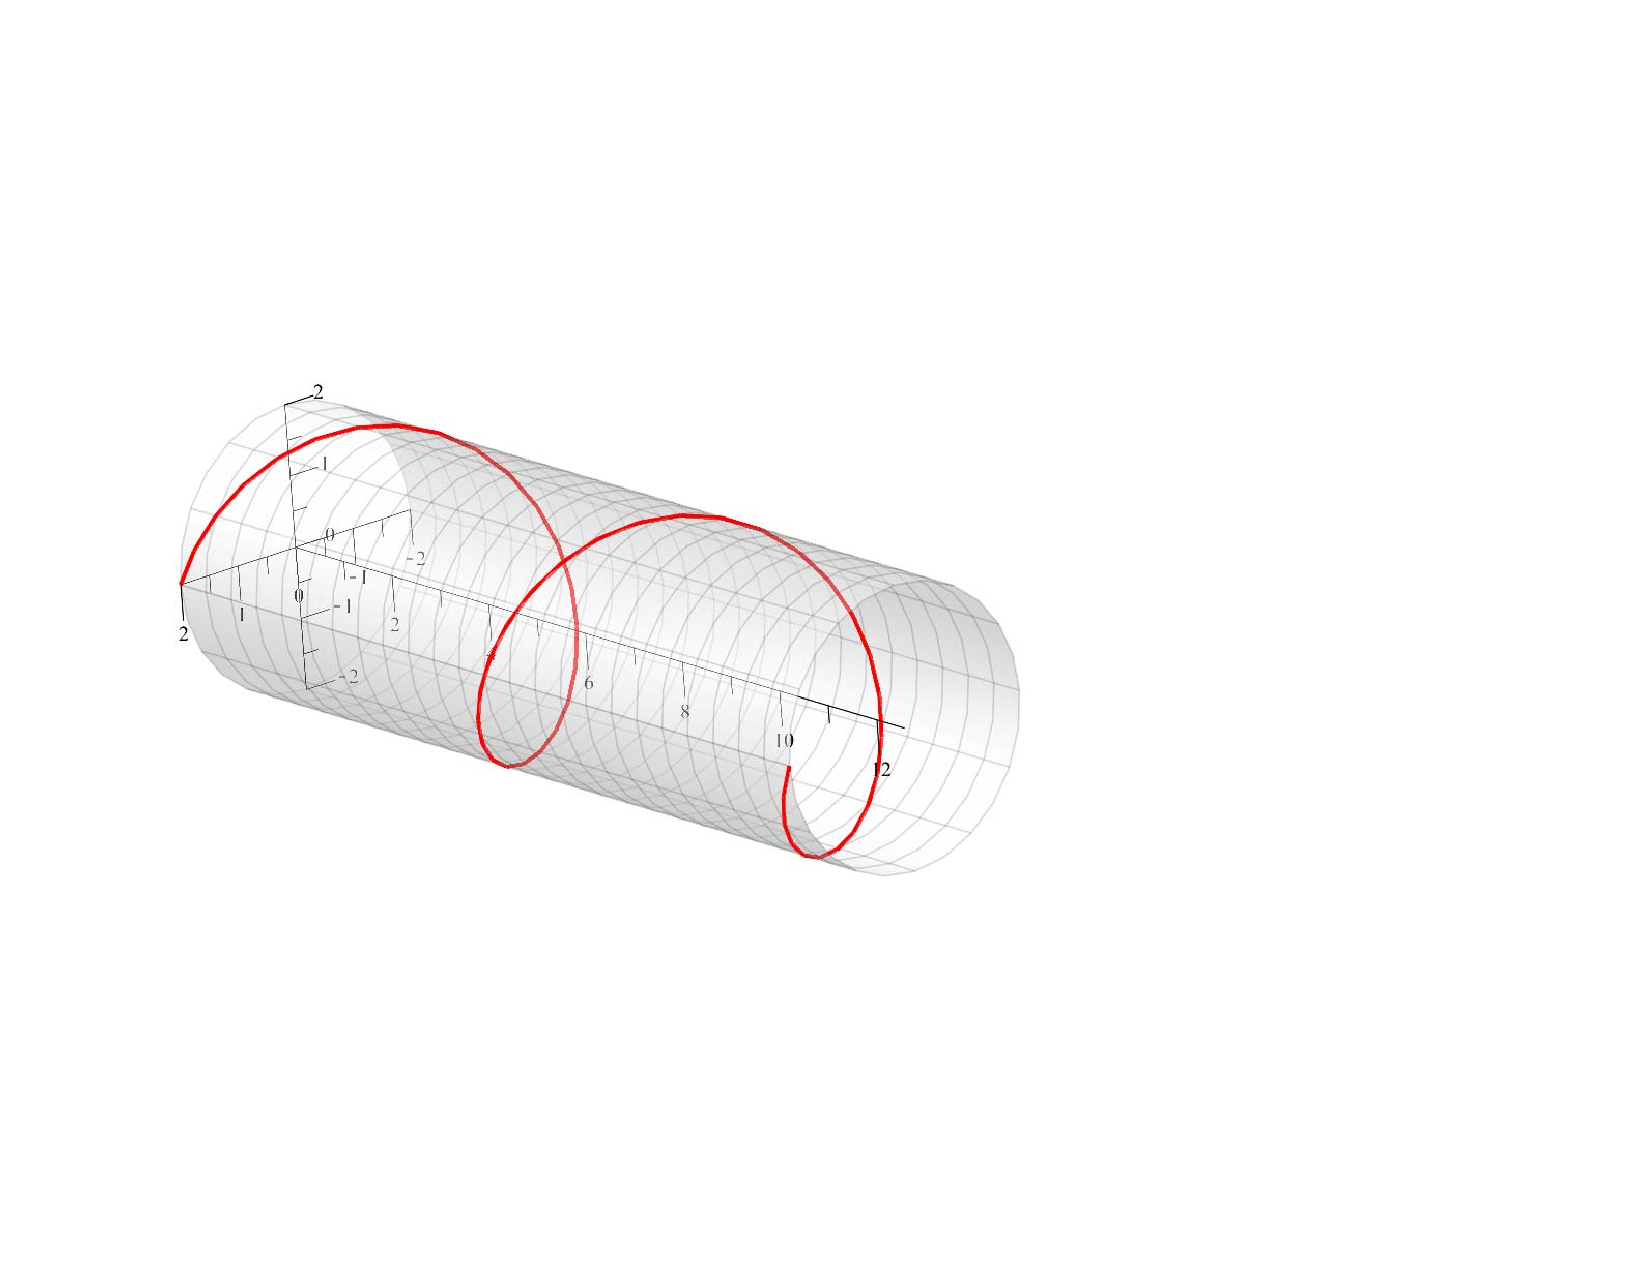
\includegraphics[scale=0.5]{helix.pdf}
\end{center}

Compute the unit tangent, principal unit normal, and binormal vectors ${\bf T}(t)$, ${\bf N}(t)$, and ${\bf B}(t)$.\\

NOTE: Here is a sketch of the helix from problems 17b with the ${\bf TNB}$-Frame (Frenet Frame) represented at four different points.
\begin{center}
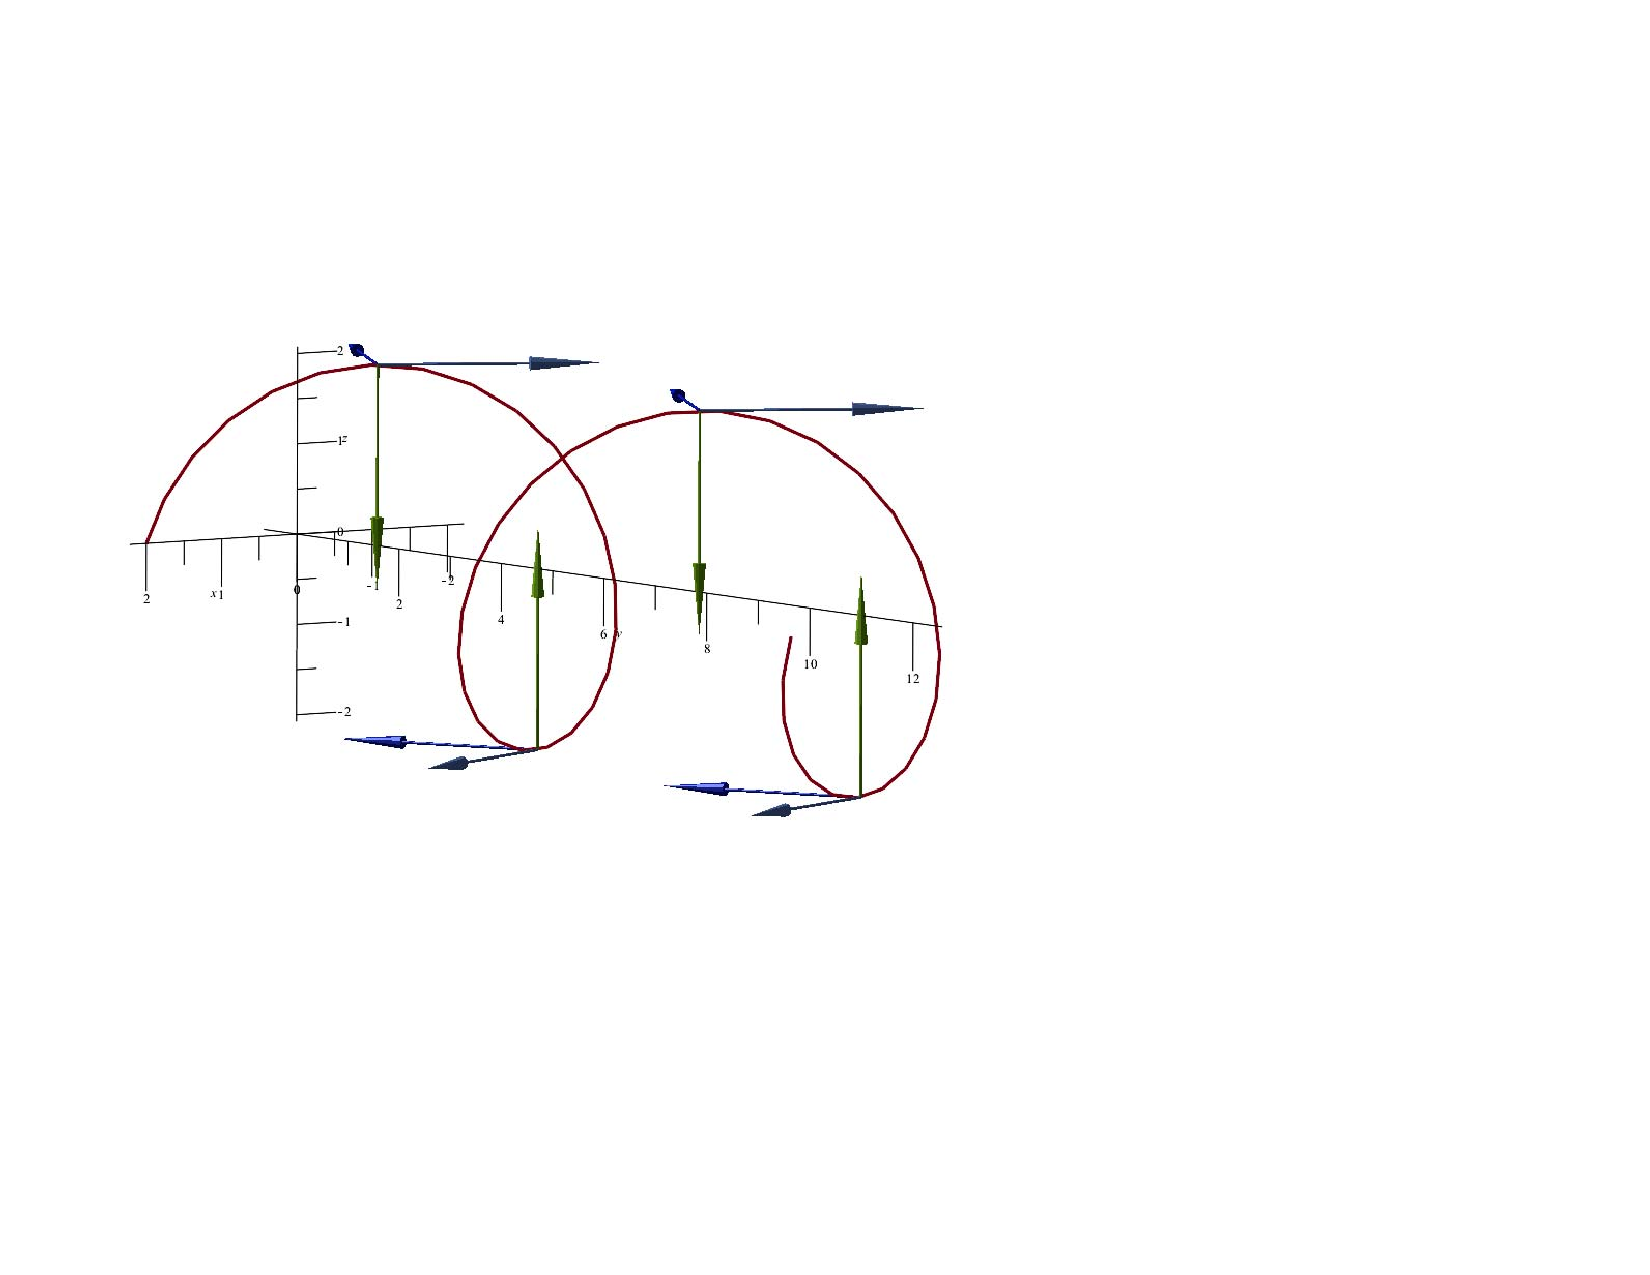
\includegraphics[scale=0.5]{frenet.pdf}
\end{center}

\ifans{\fbox{\parbox{1\linewidth}{${\bf T}(t)=\left\langle -\frac{2}{\sqrt{5}}\sin{t}, \frac{1}{\sqrt{5}}, \frac{2}{\sqrt{5}}\cos{t}\right\rangle$; ${\bf N}(t)=\left\langle -\cos{t}, 0, -\sin{t}\right\rangle$; \\
${\bf B}(t)=\left\langle -\frac{1}{\sqrt{5}}\sin{t}, -\frac{2}{\sqrt{5}}, \frac{1}{\sqrt{5}}\cos{t}\right\rangle$\\
}}} \fi

\item  \emph{{\bf Definition:} The plane determined by the unit tangent and normal vectors ${\bf T}$ and ${\bf N}$ at a point $P$ on a curve $C$ is called the {\bf osculating plane} of $C$ at $P$.  From the latin ``Osculum," meaning to kiss, this is the plane that comes closest to containing the part of the curve near $P$.}\\

Compute an equation of the osculating plane of the helix from part (b) at the point which corresponds to $t=\pi$.\\

\ifans{\fbox{$2y+z=2\pi$}} \fi

\item \emph{{\bf Definition:} The plane determined by the unit normal and binormal vectors ${\bf N}$ and ${\bf B}$ at a point $P$ on a curve $C$ is called the {\bf normal plane} of $C$ at $P$.  It consists of all lines that are orthogonal to the tangent vector ${\bf T}$.}\\

Compute an equation of the normal plane of the helix from part (b) at the point which corresponds to $t=\pi$. \\

\ifans{\fbox{$y-2z=\pi$}} \fi

\end{enumerate}

\end{enumerate}

\end{document}